\begin{table}
\begin{center}
\caption{ Wyznaczone wartośc prądu progowego $I_0$ w różnych temperaturach $T$ dla lasera krawędziowego 635\,nm. }
\begin{tabular}{ | C{3.5cm}|  C{3.5cm} | C{3.5cm} | C{3.5cm}|}
\hline
$T$ [K] &   $I_{th}$ [mA]   \\ \hline
293      &   22.4 $\pm$ 0.3  \\ \hline
298      &   25.0 $\pm$ 0.2  \\ \hline
303      &   28.1 $\pm$ 0.3  \\ \hline
308      &   31.3 $\pm$ 0.6  \\ \hline
313      &   35.7 $\pm$ 0.9  \\ \hline
\end{tabular}
\end{center}
\end{table}
\begin{figure}
\center
  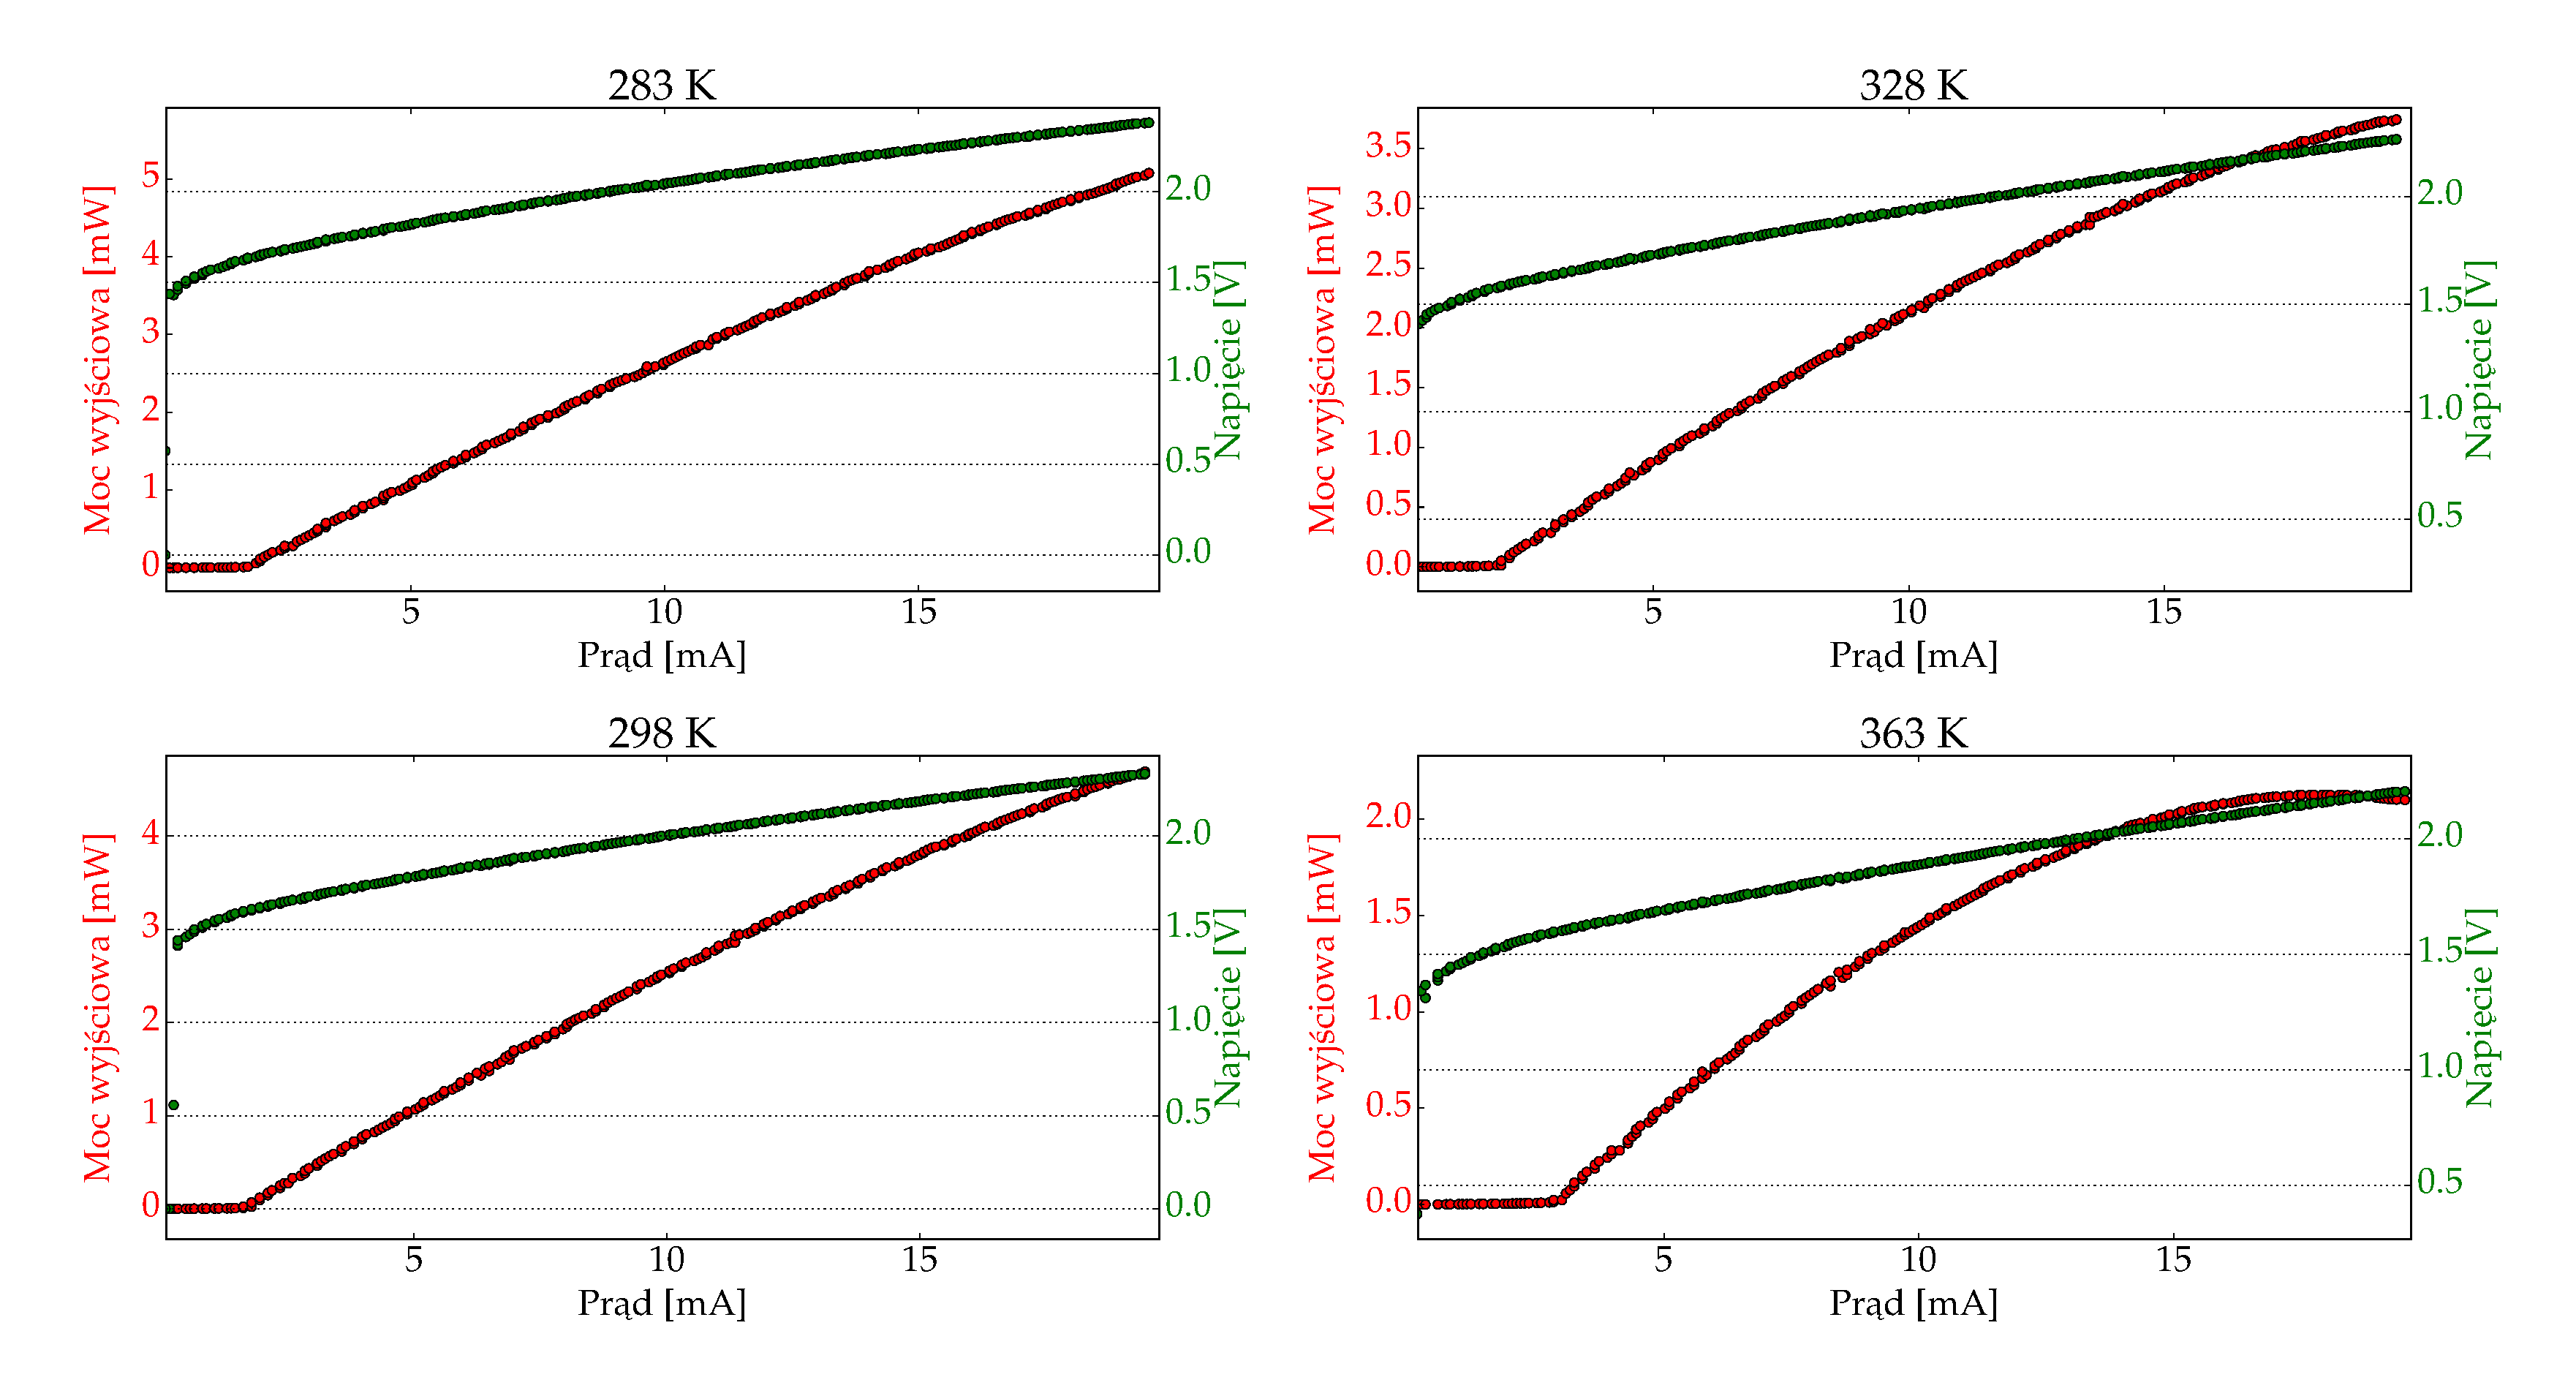
\includegraphics[scale=0.30]{plot635/plot_ivl_4.eps}
  \label{rys1}
  \caption{Wykres napięcia i mocy od prądu.} 
\end{figure}
\begin{figure}
\center
  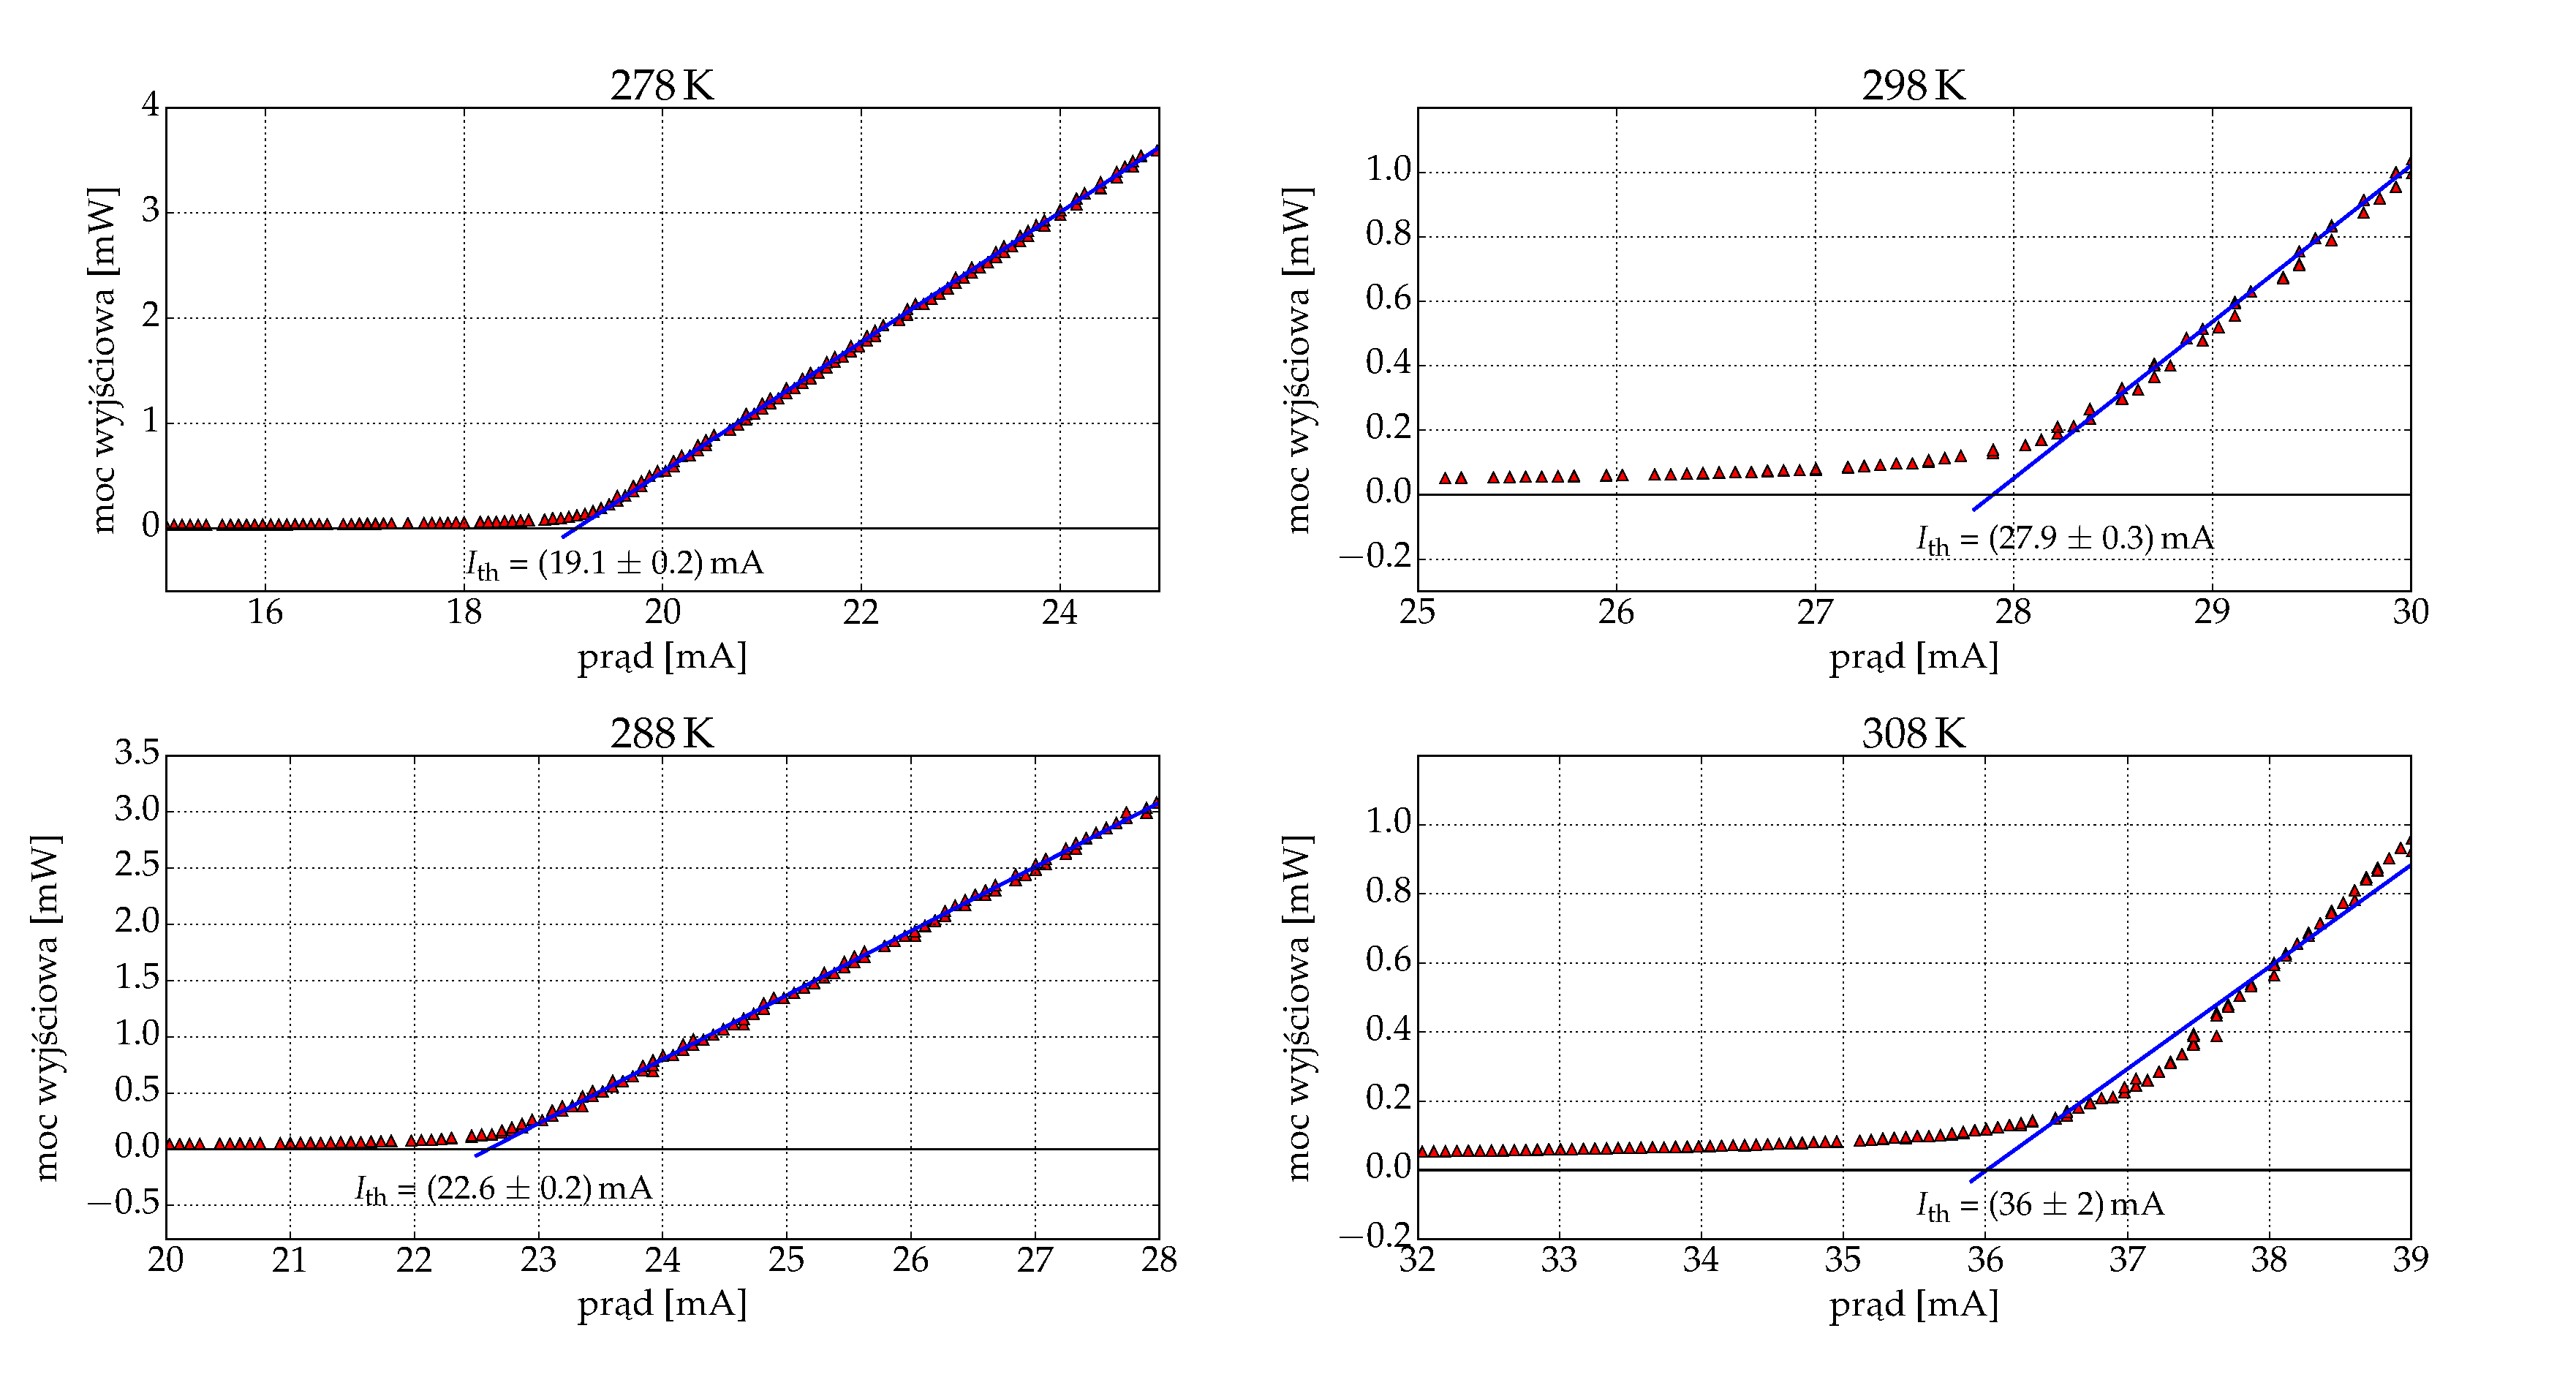
\includegraphics[scale=0.30]{plot635/plot_i_th_4.eps}
  \label{rys2}
  \caption{Wykres prądu progowego.}
\end{figure}
